\documentclass{my_cv}
%\usepackage{showframe}

\usepackage[danish]{babel} 
\usepackage[utf8]{inputenc}


%\usepackage[applemac]{inputenc}

\begin{document}
\firstpagestyle{\contact{Engvej 251}{9440 Aabybro}{privat@jossound.dk}{+45 40 15 82 36}}
%
\noindent

    \vspace*{4pt}
    \name{Jonas Flensborg Riis Buchholdt - CV}
    \vspace{10pt}
	\degree{Cand. Polyt. i akustik og signalbehandling}
	%
	\begin{minipage}[t]{.75\textwidth}%
    %\vspace{4pt}
    Jeg er uddannet som Cand. Polyt. i akustik og signalbehandling. Jeg har altid interesseret mig forstærkere og højttalere og akustik. Mit masterprojekt gik ud på, at skabe et jævnt lydtryk, og ensartet frekvens respons i bevægende atmosfæriske tilstande. Grundet min store interesse indenfor emnet, har jeg opbygget et udlejnings- og akustik rådgivningsfirma under mine studier. Dette har givet mig rigtig mange erfaringer omkring, hvordan folk oplever selve lyden, og hvad der skal til for, at folk får en god lydoplevelse.

\end{minipage}
\hfill%
\begin{minipage}[t][0.20\textwidth][b]{.20\textwidth}
	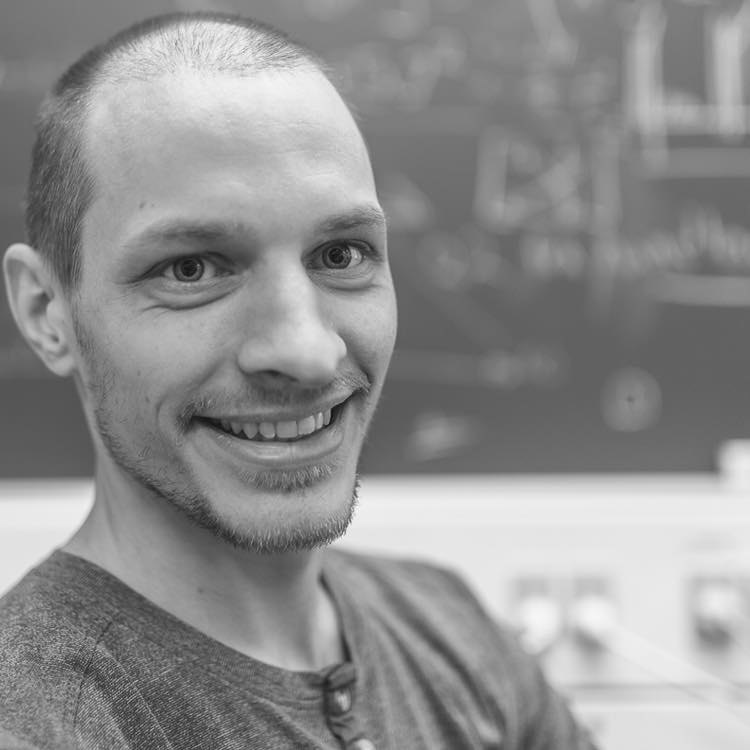
\includegraphics[width=\textwidth]{figures/mig.jpg}
\end{minipage}%
%
\section{Uddannelse}
\datedsubsection{2017--2019}{Civilingeniør i akustik og signalbehandling (AAU)}
%
\begin{focusTable}
	& Forskning og udvikling inden for hardware, akustik og audio industrien.\\
	& Gruppearbejder, struktureret tværfagligt samarbejde og selvstændigt arbejde.\\
	& Tage ansvar for egen professionel udvikling og specialisering.
\end{focusTable}
%
\project{10}{Adaptiv optimering af SPL i bevægelig atmosfære.}
\begin{projectTable}
	Metode(r) 	& Teori indenfor lydens udbredelse i bevægelig atmosfære \\
				& Impulsrespons via statistisk tids synkronoseret sine sweep målinger\\
				& Programmering af måleprogram i MATLAB\\
				& Akustiske målinger i lyddøt rum, i vindtunnel og udendørs
\end{projectTable}
%
\project{9}{Taleforståelses differense mellem airborn og bone born lyd.}
\begin{projectTable}
	Metode(r)	& Måling af psykometrisk funktion på testpersoner\\
				& Hint metoden\\
				& Programmering af test signal i Matlab\\
				& Programmering af estimeringsfunktioner i Matlab
\end{projectTable}
%
\project{8}{Optimering af FIR filter til direktionaliteten på cardioid low frequency højttaler.}
\begin{projectTable}
	Metode(r)	& Måling og modulering af given transducer\\
				& Design og konstruktion at kabinet\\
				& Design og Programmering af genetiske algoritmer\\
				& Design a test i lyddøt rum\\
\end{projectTable}
%
\project{7}{Statistisk Identificering af alarmer.}
\begin{projectTable}
	Metode(r) 	& Statistiske korrelations metoder til Identificering af periodiske signaler\\
				& Måling af alarmer i støjende omgivelser\\
				& Programmering af test i Matlab
\end{projectTable}
%
\datedsubsection{2014--2017}{Bachelor i Elektronik og IT (AAU)}
\begin{focusTable}
				& Analog og digital elektronik.\\
				& Udvikling af software, herunder samspil med hardware.\\
				& Metoder og redskaber til at beskrive, analysere, modellere, implementere, teste og dokumentere elektroniske systemer på et videnskabeligt grundlag.\\
				& Teorier og metoder, der indgår i indlejrede realtids signalbehandlingssystemer.
\end{focusTable}
%
\project{6}{Guitar effekter.}
\begin{projectTable}
	Metode(r)	& DSP\\
				& Assembler med både enkelt og dobbelt præcision\\
				& Realtids processering
\end{projectTable}
%
\project{5}{Autonom grasslåmaskine styret via differentiale GPS.}
\begin{projectTable}
	Metode(r)	& Mikroprocessor\\
				& FPGA programmering\\
				& GPS signaler\\
				& Wi-Fi
\end{projectTable}
%
\project{4}{Kelvin kontrol af LED array baseret på lyset udefra.}
\begin{projectTable}
	Metode(r)	& FPGA\\
				& WHDL\\
				& Design af ekstern hardware moduler\\
\end{projectTable}
%
\project{3}{Klasse H forstærker.}
\begin{projectTable}
	Metode(r)	& Strømspejl\\
				& Konstantstrømsgenerator\\
				& Lydsignalsstyret strømforsyning som følger output signalet\\
				& Tilbagekobling\\
				& Analog filtre\\
				& Design af hardware\\
				& Simulering af hardware		
\end{projectTable}
%
\project{2}{Lokaliseringsenhed ved hjælp af lyd.}
\begin{projectTable}
	Metode(r)	& Mikroprocessor\\
				& Fase forskel på lydsignaler\\
				& C programmering\\
				& Aktuatorstyring\\
\end{projectTable}
%
\project{1}{Elektronisk nødstop på roterende værktøj.}
\begin{projectTable}
	Metode(r)	& Mikroprocessor\\
				& C programmering\\
				& Hardware design\\
				& PCB
\end{projectTable}
%
\datedsubsection{2009--2013}{Elektronik fagtekniker  (EUC syd) ved LINAK A/S}
\begin{focusTable}
				& Analog og digital elektronik\\
				& HF kredsløb\\
				& Forsærker, SMPS og linear strømforsynings kredsløb\\
				& Fejlfinding af hardware\\
				& Metoder til test og beregning af grundlæggende elektronik\\
\end{focusTable}
%
\section{Erhvervserfaring}
\datedsubsection{2019--2019}{Rådgiver ved RTX i focusgruppe.}
\begin{focusTable}
	& Rådgivning omkring sammenspil blandt elektronik og brug af elektronik i tidspressede siturationer \\
	& Metoder til bedre design af funktionaliteten af trådløse systemer til PA og musik instrumenter \\
\end{focusTable}
%
\datedsubsection{2009--2019}{Akustik rådgiver, Ejer af Jossound.}
\begin{focusTable}
	& Udlejning af lyd \\
	& Rådgivning indenfor lyd og akustik \\
	& Test af nye teorier \\
\end{focusTable}
%
\datedsubsection{2009--2013}{Elektronik fagtekniker, Lærling ved LINAK A/S}
\begin{focusTable}
	& Komponent optimering \\
	& Fejlfinding på elektronik\\
	& Design af elektronik\\
\end{focusTable}
%



%
\section{IT}
%
\newlength{\columnWidth}
\setlength{\columnWidth}{\dimexpr(\textwidth/3)\relax}
\begin{tabular}{p{\columnWidth} p{\columnWidth} p{\columnWidth}}
	\skill{Python}{4} 	& \skill{Altium}{3}	& \skill{Word}{5} 		\\
	\skill{Matlab}{5}	& \skill{Mentor PCB}{3}	& \skill{Excel}{5}		\\
	\skill{C}{4}		& \skill{OrCad}{2}		& \skill{powerpoint}{5} \\
	\skill{Assembler}{4}& \skill{Labview}{2}		& \skill{Latex}{5}		\\
	\skill{WHDL}{4}		& \skill{LT Spice}{4}	&						
\end{tabular}
%

\section{Sprog}
\begin{tabular}{l}
	\skill{Dansk}{5} \\
	\skill{Engelsk}{5} \\
	\skill{Tysk}{2}
\end{tabular}

\section{Personlig}
Jeg bor sammen med min kone, Heidi på en land ejendom, som vi løbende renoverer. Derudover går jeg til koncerter, som tilskuer og lydinginør ved pulten. Jeg værdsætter min familie højt, da det giver mig glæde og inspiration til hverdagen. 
Vi kan godt lide at være sammen og gå tur in naturen med vores hund.  Jeg har derudover altid interreseret mig for gymnastik, og har gået til springgymnastik og powertumbling siden jeg var 8 år. 

%	
\end{document}
